%sse
\documentclass[../../main/main.tex]{subfiles}


\begin{document}
\title{Systems Security Engineering}


%%%%%%%%%%%%%%%%%%%%% Chapter CSBD ACL %%%%%%%%%%%%%%%
\chapter{Systems Security Engineering \& Patrol Base Operations}\label{chp:sse}


       %%%%%%%%%%%%%%%%%% Section Systems %%%%%%%%%%%%%%%%
\section{The Systems Perspective}\label{sec:systems}
A system is a set of interacting and interdependent components that act as a whole to perform some behavior or function.  Examples of systems include the human body, socio-political systems, and computer systems. 

The patrol base operations satisfy this definition of a system.  As a whole, the patrol base operations perform some function(s).  This function is described in the Ranger Handbook \cite{rangermanual} and discussed in section \ref{sec:pb}.  The patrol base operations are comprised of interdependent and interacting components.  In general these components are the individual soldiers.  But, the way this master thesis defines the patrol base operations, the definition of a component varies.

This master thesis defines the patrol base operations as a system of systems.  More specifically, this thesis models the patrol base operations as a hierarchy of \glsentrylongpl{ssm}.  Chapter \ref{chp:ssmmodel} describes \glsentryshortpl{ssm} in general.   Section \ref{sec:modelingpb} describes this model of the patrol base operations.  This model presents the patrol base operations as a hierarchy wherein each level of the hierarchy represents a decreasing level of abstraction.   

At the top and most abstract level, the components are phases of the patrol base operations.  These phases commence in a sequential order to achieve the goal of the patrol base operations.  Each lower level of the hierarchy is composed of less abstract phases. At each level, the components function sequentially (typically) to achieve the ultimate goal.  

This system of system also contains non-hierarchically defined components.  For example, an escape-level component models situations wherein the patrol base operations are aborted.  The escape level component is reachable from any component at any level of the hierarchy.  Soldiers also function within this system of systems in a non-hierarchical manner.  However, soldiers were not modeled in detail for this master thesis.  Nevertheless, they were discussed in detail and ready to be modeled.

In this way, the patrol base operations represent a system and are amiable to the systems engineering perspective.  

     %%%%%%%%%%%%%%%%%% Section Systems Engineering %%%%%%%%%%
\section{Systems Engineering}\label{sec:se}
Systems engineering is an interdisciplinary approach aimed at solving problems involved in the design, development, realization, and life-cycle maintenance of systems.
  
  
 This master thesis focuses on the design phase of systems engineering.   The aim is to model the patrol base operations in a manner that is amiable to verifying specific security properties of the system.  Specifically, the patrol base operations must satisfy the property of complete mediation. 


But, this thesis does not aim to build a new system.  Rather this thesis remodels an existing system.   This is necessary because the goal of this thesis is to determine whether or not it is possible to verify the specific security properties on the subclass of systems that we are exploring.  Most people would agree that testing a new method on a new system would be unwise.  This is why this thesis did not do that.    


This approach has the side-effect of also demonstrating CSBDs utility in the life-cycle phase of systems engineering.  It follows readily from the news today that many systems were not designed with security in mind.  Eliminating already-in-use systems and legacy systems may not always be practical or desirable.  Nevertheless, security remains an important aspect of system performance.  This, in part, justifies a re-look at (or remodeling of)  of an already existing system.


There are additional benefits to systematically modeling the patrol base operations in a way that is amiable to formal verification.  This type of thinking provides new insights and suggests areas for improvement\footnote{The subject matter expert who focused on the details of the patrol base operations also noted areas for improvement.  He was not available to provide details at the writing of this master thesis.}.  This is a known benefit.  For example, Wikipedia \cite{wikiformalmethods} notes that "Sometimes, the motivation for proving the correctness of a system is not the obvious need for reassurance of the correctness of the system, but a desire to understand the system better."  A greater understanding of a system applies to all phases of systems engineering.

     %%%%%%%%%%%%%%%%%% Section Systems Security Engineering %%%%%%
\section{Systems Security Engineering}\label{sec:sse}

  In general, the CSBD approach to verifying these security properties is a design phase activity.  This is because it is well established that the best way to apply security to a system is to engineer the system with security in mind at the design phase.  

\subsubsection{Systems Security Engineering Framework}\label{sssec:sseframework}

\begin{figure}[ht]
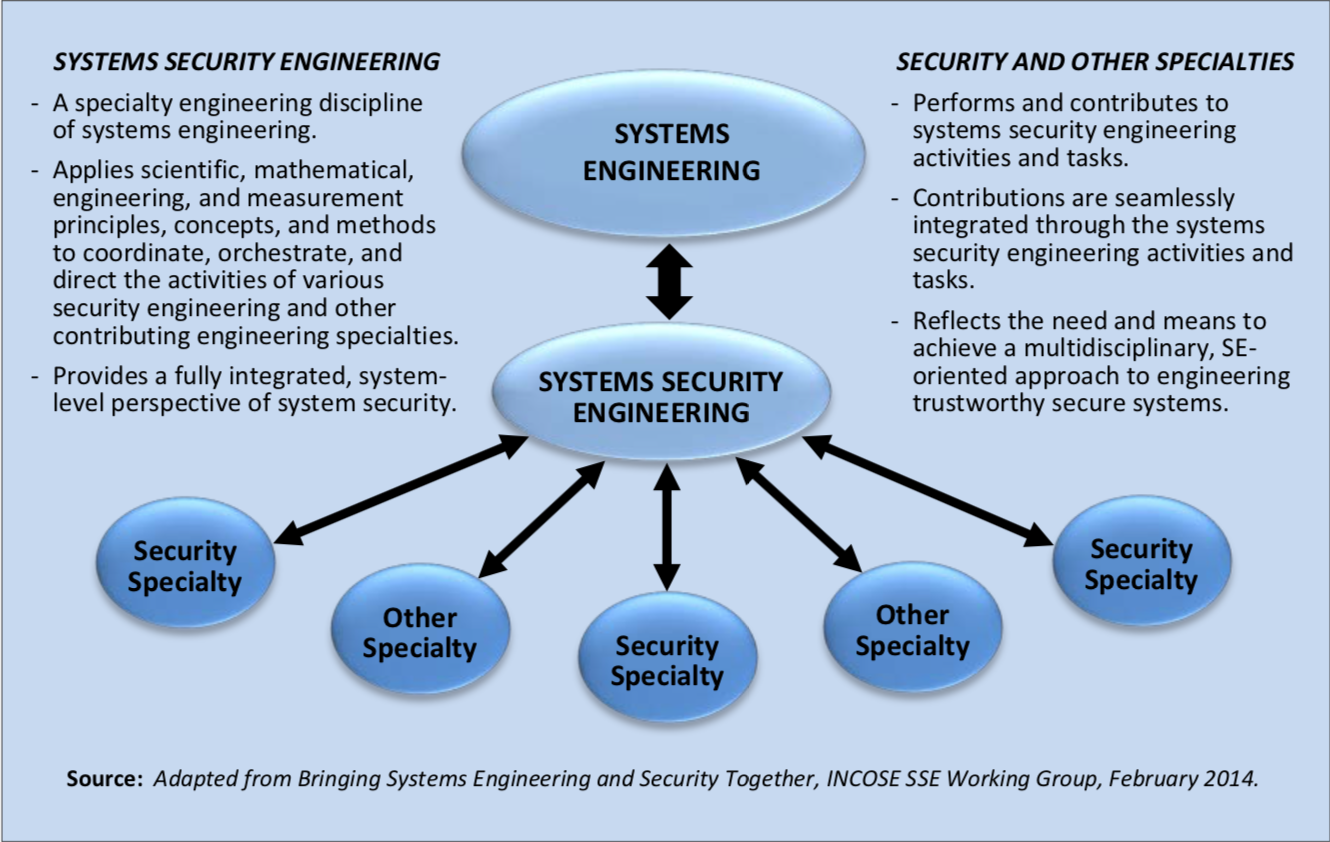
\includegraphics[width=\linewidth]{../figures/seincontext.png}
\caption{This is a clip from NIST 800-160.}
\label{fig:nist800160}
\end{figure}

This is some text after the figure.

\subsection{Trustworthiness}\label{ssec:trustworthiness}
\subsubsection{Complete Mediation}\label{sssec:completemediation}

\subsection{Verification}\label{ssec:verification}
\subsection{Documentation}\label{ssec:documentation}
\subsection{Reproducibility}\label{ssec:reproducibility}

      %%%%%%%%%%%%%%%%%%% Section Verification & Documentation %%%%%%
\section{Verification \& Documentation}

      %%%%%%%%%%%%%%%%%%% Section Complete Mediation %%%%%%%%%%%
\section{Principle of Complete Mediation}

\subsection{Formal Verification Using Computer-Aided Reasoning}

\end{document}